\section{Introduction}

\subsection{A quoi sert ce logiciel}
Ce logiciel est un \acc{gestionnaire de questions Flash}. 

Il permet de :
\begin{tcbenumerate}
    \tcbitem Créer des fichiers \frquote{\LaTeX} basés sur un \acc{modèle} adapté pour la \acc{présentation en classe}. 
    \tcbitem Organiser ces fichiers dans un répertoire, et permettre un accès facile à l'enseignant. 
    \tcbitem Charger des questions prédéfinies par l'application \frquote{implementer\_enonce}.
    \tcbitem Compiler les documents et les organiser par année - mois - date prévue de projection. 
    \tcbitem Construire des évaluations par choix aléatoire de questions durant une période donnée.
\end{tcbenumerate}

Cela permet une gestion fine des projections d'automatismes en classe. 

L'enseignant peut simplement \acc{choisir} dans un corpus de modèles, les questions qu'il souhaite projeter. 

Cela permet d'\acc{adapter} les questions projetées au niveau de la classe et aux \acc{objectifs} de l'enseignant. 


\subsection{Comment l'utiliser}

Dans le répertoire courant de l'application, toutes les manipulations à effectuer sont données dans le fichier \acc{README.md}

Des \acc{scripts d'installation et de lancement}  ont été prévues, et nécessitent une distribution \acc{Python} comportant la librairie \acc{tcl} binaire. 

Tester avec votre distribution, et si ça ne fonctionne pas, demander à un agent IA de vous dire quelle version télécharger pour être compatible. 

\newpage
\subsection{Architecture}

Le projet s'organise selon l'arborescence suivante :

\begin{center}
\begin{minipage}{0.8\textwidth}
\dirtree{%
.1 QFGen/.
.2 databases/.
.3 database\_6eme/.
.4 database\_2025\_1.json.
.4 database\_2025\_2.json.
.4 \ldots.
.3 database\_5eme/.
.3 database\_4eme/.
.3 \ldots (un dossier par niveau).
.2 generated/.
.3 tex/ (fichiers \LaTeX{} générés).
.4 6ème/.
.5 2025/.
.6 09/.
.6 10/.
.3 pdf/ (PDF compilés).
.3 eval\_tex/ (évaluations \LaTeX).
.3 eval\_pdf/ (évaluations PDF).
.2 qf\_gen\_config/.
.3 api\_key.txt (clés API).
.3 ai\_provider.txt (choix IA).
.3 prompts.txt (prompts IA).
.3 cfg.py (configuration).
.2 latexhighlighter/ (coloration syntaxique).
.2 UI\_question\_loader/ (interface de chargement).
.2 main.py (interface principale).
.2 auto\_question\_maker.py (génération IA).
.2 modele\_QF.tex (modèle questions).
.2 Modele\_QF\_eval.tex (modèle évaluations).
}
\end{minipage}
\end{center}

\subsubsection{Modules principaux}

\begin{tcbenumerate}
    \tcbitem \textbf{main.py} : Interface graphique principale (CustomTkinter). Gère les 3 questions par série, la sélection de classe/date, la compilation LaTeX.

    \tcbitem \textbf{auto\_question\_maker.py} : Module de génération automatique via IA (OpenAI ou Claude). Permet de générer question, réponse détaillée, réponse courte et thème.

    \tcbitem \textbf{question\_manager.py} : Gestion de la base de données JSON des questions par niveau et par période.

    \tcbitem \textbf{latexcompiler.py} : Compilation LaTeX avec LuaLaTeX, gestion des fichiers auxiliaires et ouverture automatique des PDF.

    \tcbitem \textbf{latexhighlighter/} : Coloration syntaxique en temps réel, vérification de syntaxe LaTeX, et visualisation PDF intégrée.

    \tcbitem \textbf{UI\_question\_loader/} : Interface de navigation dans les bases de données pour charger des questions existantes comme modèles.

    \tcbitem \textbf{tex\_eval\_maker.py} : Génération d'évaluations par sélection aléatoire de questions sur une période donnée.
\end{tcbenumerate} 


\section{Fonctionnalités}

\subsection{Vue d'ensemble de l'interface}

L'interface principale permet de gérer jusqu'à 3 questions par série de questions flash.

\begin{center}
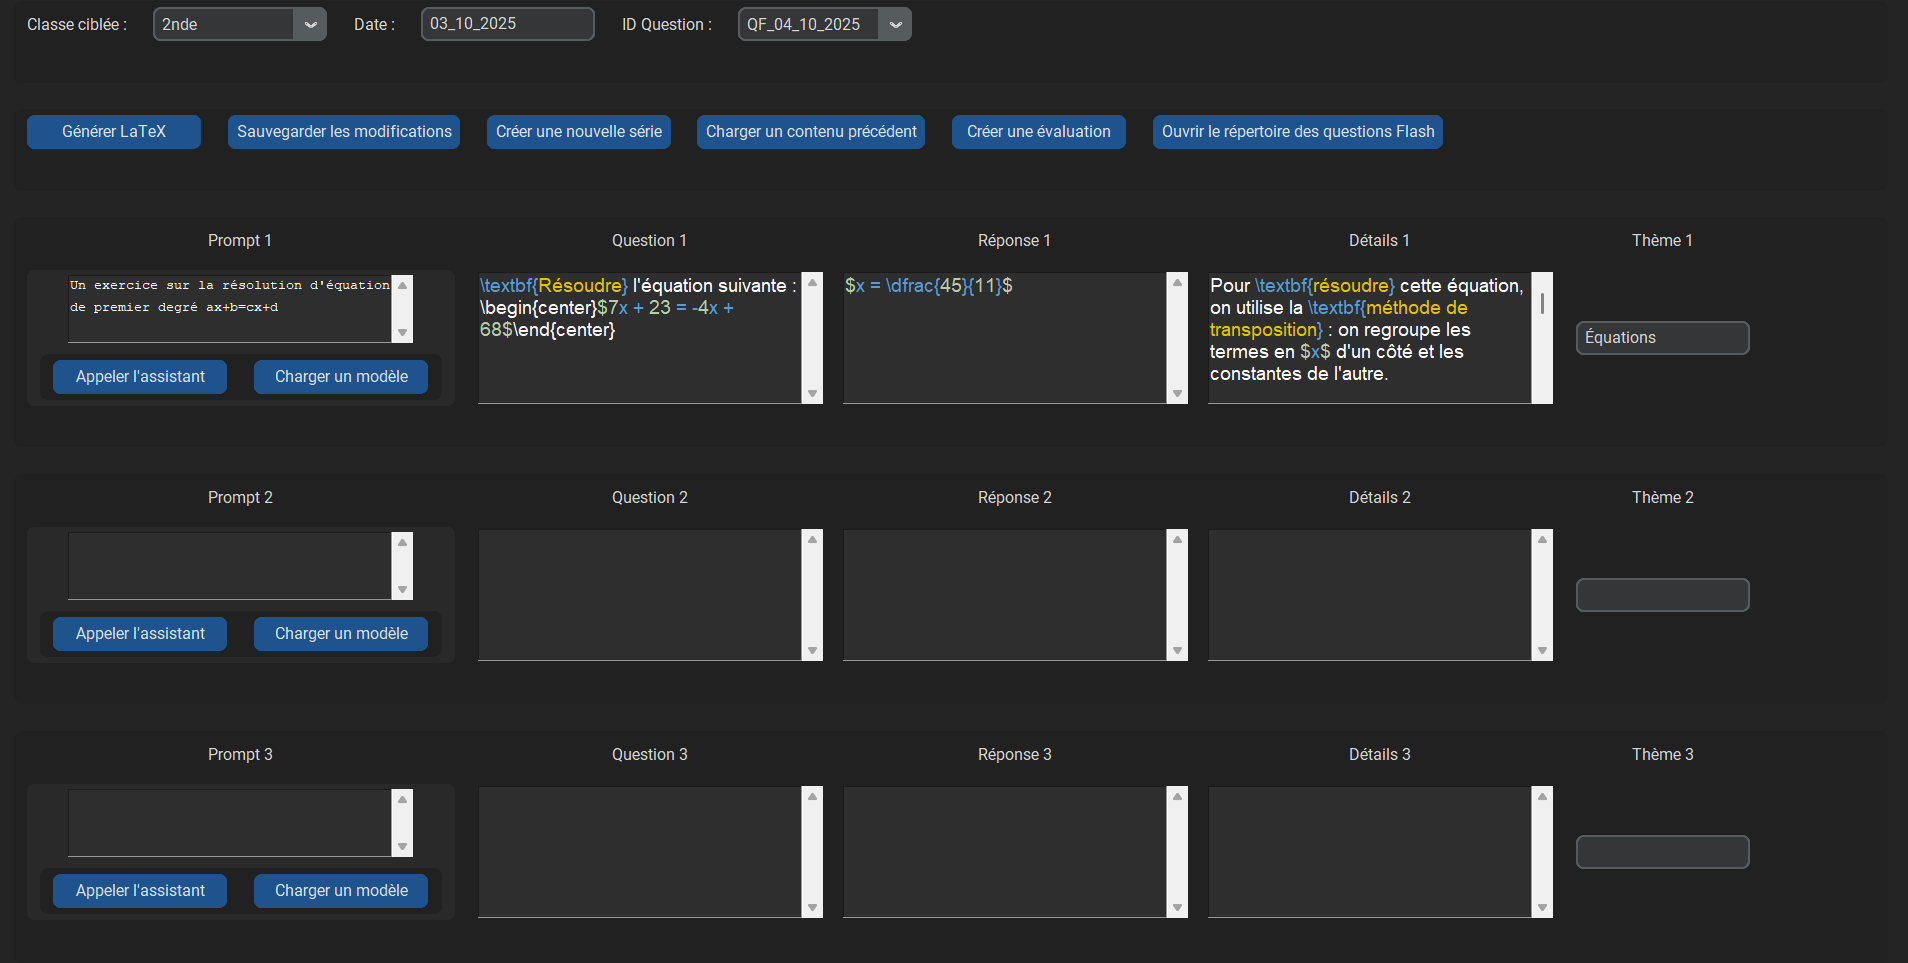
\includegraphics[width=0.95\textwidth]{images/UseCase_global.png}
\captionof{figure}{Interface principale du logiciel}
\end{center}

Pour chaque question, l'utilisateur dispose de :
\begin{tcbenumerate}
    \tcbitem Un champ pour l'\textbf{énoncé} de la question (LaTeX)
    \tcbitem Un champ pour la \textbf{réponse courte} (affichée en bas de document)
    \tcbitem Un champ pour la \textbf{réponse détaillée} (correction complète)
    \tcbitem Un champ pour le \textbf{thème} de la question
    \tcbitem Un champ \textbf{prompt} pour guider l'assistant IA
\end{tcbenumerate}

\subsection{Création d'une nouvelle série}

\subsubsection{Saisie manuelle}

L'utilisateur peut saisir directement le code LaTeX dans les champs prévus. La coloration syntaxique aide à repérer les erreurs de syntaxe.

\begin{center}
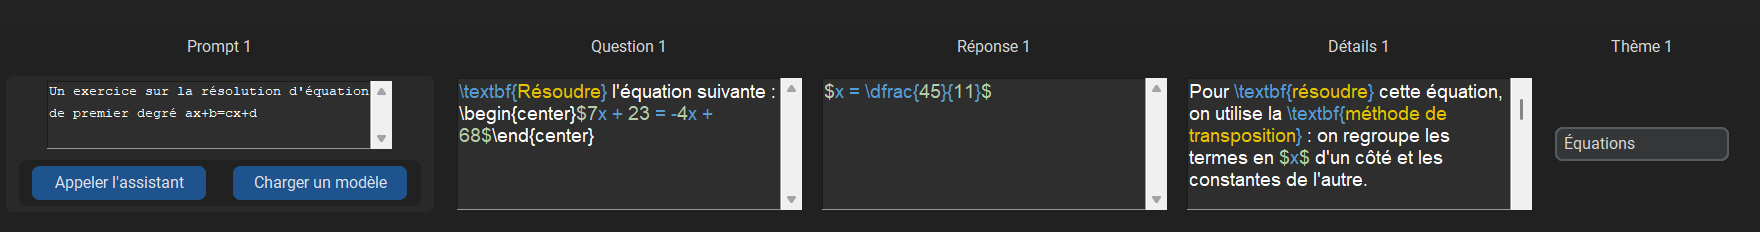
\includegraphics[width=0.75\textwidth]{images/UseCase_equation.png}
\captionof{figure}{Exemple de saisie d'une question sur les équations}
\end{center}

\subsubsection{Génération assistée par IA}

En cliquant sur \frquote{Appeler l'assistant}, le logiciel utilise l'IA configurée (OpenAI ou Claude) pour :
\begin{tcbenumerate}
    \tcbitem Générer l'énoncé à partir du prompt
    \tcbitem Générer la réponse détaillée
    \tcbitem Générer la réponse courte
    \tcbitem Proposer un thème pour la question
\end{tcbenumerate}

Le résultat s'affiche en \acc{temps réel} (streaming) dans les champs correspondants.

\subsection{Chargement de questions existantes}

\subsubsection{Charger un modèle}

Le bouton \frquote{Charger un modèle} permet de naviguer dans la base de données des questions déjà créées.

\begin{center}
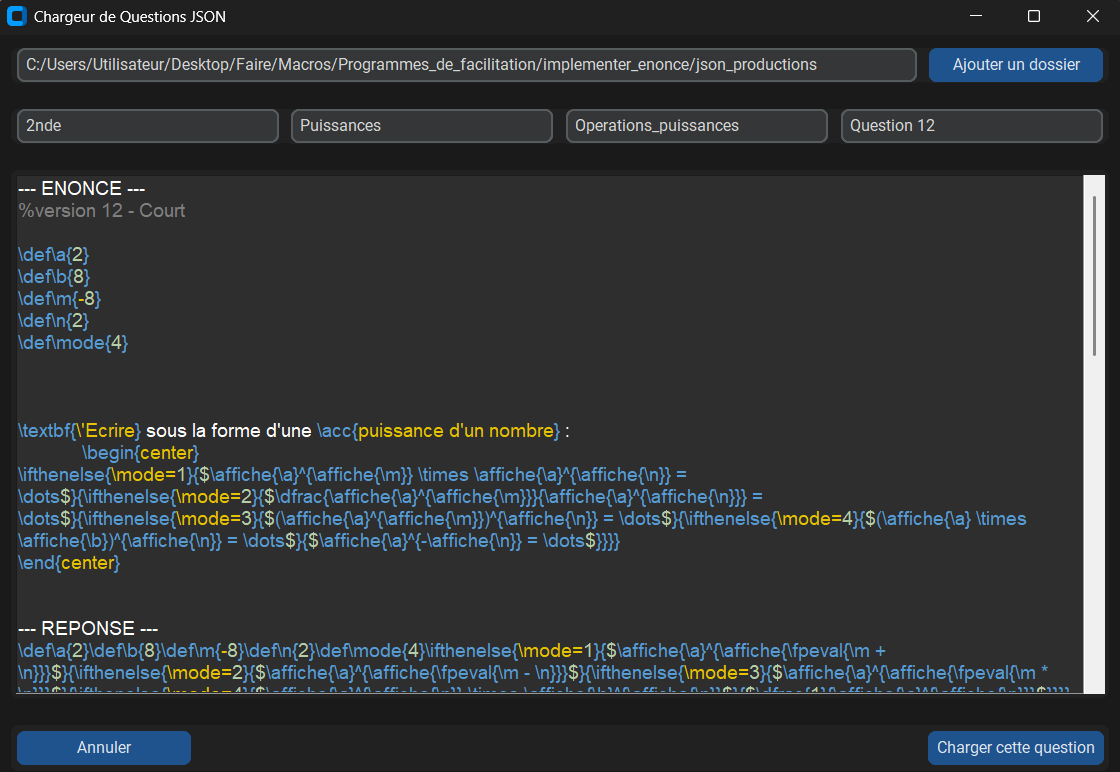
\includegraphics[width=0.85\textwidth]{images/UseCase_load_model.png}
\captionof{figure}{Interface de chargement de questions existantes}
\end{center}

L'utilisateur peut :
\begin{tcbenumerate}
    \tcbitem Parcourir les questions par \acc{niveau} (6ème, 5ème, etc.)
    \tcbitem Filtrer par \acc{thème}
    \tcbitem Prévisualiser les questions avant de les charger
    \tcbitem Charger une question comme base pour une nouvelle
\end{tcbenumerate}

\subsection{Sauvegarde et compilation}

\subsubsection{Sauvegarde dans la base de données}

Le bouton \frquote{Sauvegarder les modifications} enregistre les 3 questions dans la base de données JSON correspondant au niveau et à la date sélectionnés.

Format : \texttt{databases/database\_\{classe\}/database\_\{année\}\_\{mois\}.json}

\subsubsection{Génération LaTeX et compilation}

Le bouton \frquote{Générer LaTeX} :
\begin{tcbenumerate}
    \tcbitem Crée le fichier \texttt{.tex} à partir du modèle \texttt{modele\_QF.tex}
    \tcbitem Le place dans \texttt{generated/tex/\{classe\}/\{année\}/\{mois\}/}
    \tcbitem Lance la compilation avec LuaLaTeX
    \tcbitem Place le PDF dans \texttt{generated/pdf/\{classe\}/\{année\}/\{mois\}/}
    \tcbitem Ouvre automatiquement le PDF généré
\end{tcbenumerate}

\subsection{Création d'évaluations}

Le bouton \frquote{Créer une évaluation} permet de générer une évaluation par sélection aléatoire :

\begin{tcbenumerate}
    \tcbitem Sélectionner le \acc{niveau} concerné
    \tcbitem Définir une \acc{période} (date min - date max)
    \tcbitem Choisir le \acc{nombre de questions} à inclure
    \tcbitem Le logiciel sélectionne aléatoirement des questions dans cette période
    \tcbitem Génère un document d'évaluation avec le barème de points
\end{tcbenumerate}

Les évaluations sont enregistrées dans \texttt{generated/eval\_tex/} et \texttt{generated/eval\_pdf/}.

\section{Utilisation personnalisée}

\subsection{Modifier le modèle}

Il est possible de modifier le fichier \frquote{modele\_QF.tex} ou \frquote{Modele\_QF\_eval.tex} pour adapter à votre présentation ou utiliser vos propres packages pour la génération des documents.

\subsection{Configuration du chemin des images}

\encadrer[red]{Pour que les images s'affichent correctement dans vos documents}, vous devez configurer le chemin vers le dossier \texttt{images/} dans votre entête de modèles.

Vous pouvez : Utiliser le paramètre bfcours \texttt{dbIconPath} :

\begin{lstlisting}[language=TeX]
\dbIconPath{C:/chemin/vers/vos/images/}
\end{lstlisting}

\textbf{Remarque :} Utilisez des barres obliques \texttt{/} (slash) plutôt que des antislash \texttt{\textbackslash} pour la compatibilité LaTeX, même sous Windows.

\acc{Vérification} :

Pour vérifier que le chemin est correctement configuré, compilez un document contenant une image de test. Si l'image ne s'affiche pas, vérifiez :
\begin{tcbenumerate}
    \tcbitem Que le chemin est absolu (commence par \texttt{C:/} sous Windows)
    \tcbitem Que les barres obliques sont utilisées
    \tcbitem Que le dossier \texttt{images/} existe bien à l'emplacement indiqué
\end{tcbenumerate}

\subsection{Modifier les prompts}

Les prompts commencent à être un peu anciens, mais comme ils fonctionnent, je ne les modifie pas.

Vous pouvez tout à fait, à vos risques et périls, les modifier pour personnaliser l'affichage.

\subsection{Configuration de l'assistant IA}

Le logiciel supporte deux fournisseurs d'IA : \textbf{OpenAI} et \textbf{Claude (Anthropic)}.

\subsubsection{Choix du provider et du modèle}

Pour configurer le provider IA et le modèle à utiliser, éditez le fichier \texttt{qf\_gen\_config/ai\_provider.txt} :

\begin{lstlisting}
PROVIDER=claude
CLAUDE_MODEL=claude-sonnet-4-5-20250929
OPENAI_MODEL=gpt-5-2025-08-07
\end{lstlisting}

\textbf{Configuration du provider :}
\begin{tcbenumerate}
    \tcbitem Changez \texttt{PROVIDER=claude} en \texttt{PROVIDER=openai} pour utiliser OpenAI
    \tcbitem Le provider par défaut est \textbf{Claude}
\end{tcbenumerate}

\textbf{Configuration des modèles :}
\begin{tcbenumerate}
    \tcbitem \texttt{CLAUDE\_MODEL} : Modèle Claude à utiliser (défaut : \texttt{claude-sonnet-4-5-20250929})
    \tcbitem \texttt{OPENAI\_MODEL} : Modèle OpenAI à utiliser (défaut : \texttt{gpt-5-2025-08-07})
    \tcbitem Vous pouvez changer ces valeurs pour utiliser d'autres modèles disponibles
\end{tcbenumerate}

\textbf{Exemples de modèles disponibles :}

Pour Claude :
\begin{lstlisting}
claude-sonnet-4-5-20250929  (recommandé)
claude-sonnet-4-20250514
claude-3-opus-20240229
\end{lstlisting}

Pour OpenAI :
\begin{lstlisting}
gpt-5-2025-08-07  (recommandé)
gpt-4o
o3-mini
\end{lstlisting}

\subsubsection{Configuration des clés API}

Les clés API sont stockées dans \texttt{qf\_gen\_config/api\_key.txt} au format :

\begin{lstlisting}
OPENAI_API_KEY="sk-proj-xxxxx..."
ANTHROPIC_API_KEY="sk-ant-api03-xxxxx..."
\end{lstlisting}

\encadrer[red]{Conservez les guillemets autour des clés.}

\subsubsection{Avantages de chaque provider}

\textbf{Claude :}
\begin{tcbenumerate}
    \tcbitem Excellent pour les mathématiques.
    \tcbitem Meilleure compréhension du LaTeX.
    \tcbitem Réponses plus structurées.
\end{tcbenumerate}

\textbf{OpenAI :}
\begin{tcbenumerate}
    \tcbitem Intelligence améliorée ( modèle frontière ).
    \tcbitem Génération de qualité.
\end{tcbenumerate} 